\section{Synthesis theorem}
\label{sec:synthesis}

Every model with a nonempty state space has a strict hidden extension that preserves all reachable outputs and prevents exact recovery of the extended state.

\begin{theorem}[Boundary limited observer synthesis]
Let \(\Model=(X_\Model,\pi_\Model)\) be a generative model, let \(x_0\in X_\Model\) be an inhabited witness, and let \(e:O\to R\) be an admissible experiment. Then there exists a model \(\Extended\) such that:
\begin{enumerate}[label=(\roman*)]
\item \(\Extended\) is a strict latent cover of \(\Model\);
\item the empirical classes are equal, \(q_{\Emp}(\Extended)=q_{\Emp}(\Model)\), equivalently \(\Extended\approx\Model\);
\item \(\Obs(\Extended)=\Obs(\Model)\);
\item \(\Out_e(\Extended)=\Out_e(\Model)\); and
\item \(\Extended\) has no exact latent decoder.
\end{enumerate}
\label{thm:synthesis}
\end{theorem}

\begin{proof}
Choose the Boolean extension
\[
X_{\Extended}=X_\Model\times\bool
\]
and define
\[
\pi_{\Extended}(x,b)=\pi_\Model(x).
\]
Define the projection
\[
p:X_{\Extended}\to X_\Model,
\qquad
p(x,b)=x.
\]
The projection is surjective. For each \(x\in X_\Model\), the state \((x,0)\) maps to \(x\). It also preserves observation because
\[
\pi_{\Extended}(x,b)=\pi_\Model(p(x,b)).
\]
Thus \(\Extended\) is a latent cover of \(\Model\).

The cover is strict. Use the supplied witness \(x_0\in X_\Model\). Then
\[
(x_0,0)\neq(x_0,1)
\]
but
\[
p(x_0,0)=x_0=p(x_0,1).
\]
Hence the projection is noninjective.

Every latent cover is empirically equivalent to its base. Therefore
\[
\Extended\approx\Model
\]
and
\[
\Obs(\Extended)=\Obs(\Model).
\]
By empirical outcome invariance,
\[
\Out_e(\Extended)=\Out_e(\Model).
\]
Finally, the two distinct extended states \((x_0,0)\) and \((x_0,1)\) have equal observations:
\[
\pi_{\Extended}(x_0,0)=\pi_\Model(x_0)=\pi_{\Extended}(x_0,1).
\]
The extended observation map is noninjective. An exact latent decoder would imply injectivity. Therefore no exact latent decoder exists for \(\Extended\).
\end{proof}
\begin{figure}[tbp]
\centering
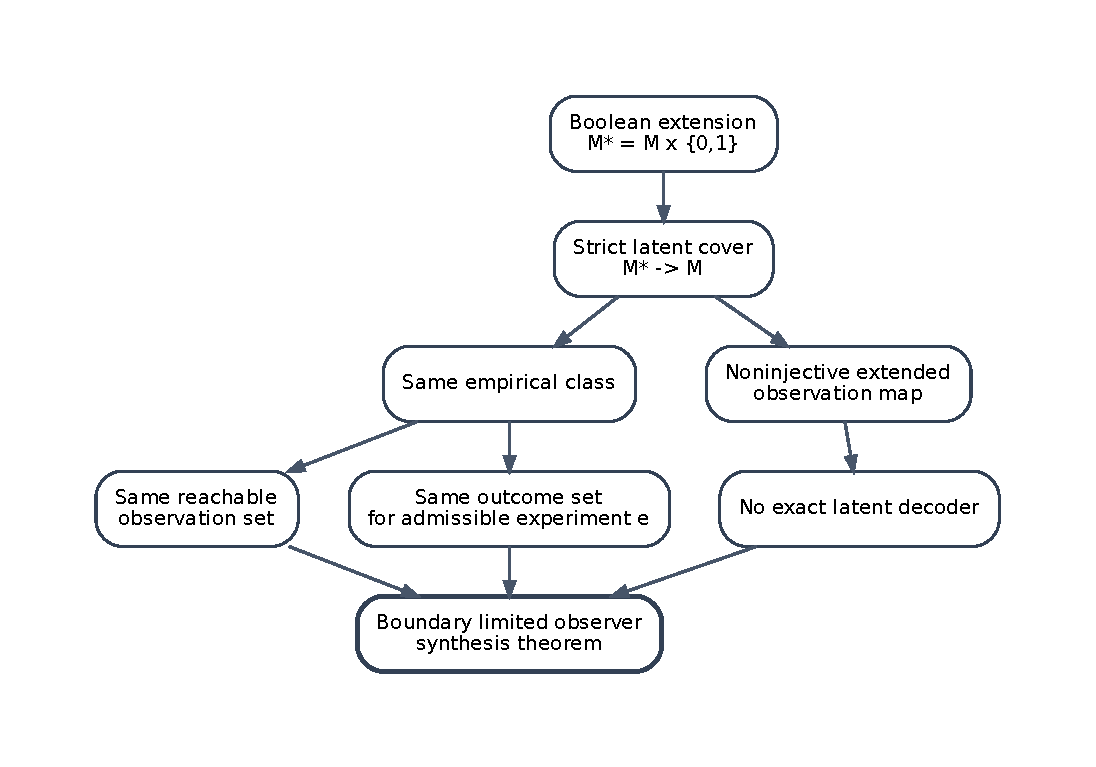
\includegraphics[width=0.82\textwidth]{figures/concept_synthesis_dependency.pdf}
\caption{Dependency structure of the synthesis theorem. The result combines fiber based reconstruction limits, model outcome invariance, strict hidden extensions, and empirical quotient structure.}
\label{fig:dependency}
\end{figure}

\subsection{Recovery from possible outputs}

The extension and its base agree on the entire reachable set. Every function of the observation, including the identity, gives the same possible outcomes. The extension always lacks an exact decoder. The base may admit one.

Uniqueness of a latent representation requires a restriction on the admissible models or a further measurement. Dynamics, causal interventions, regularity, minimality, prior probabilities, and known state counts give different restrictions. Their justification depends on the application.

\subsection{Physical interpretation}

The Boolean label provides a second representation consistent with the same outputs. A physical interpretation of that label requires independent evidence. Approximate reconstruction would require a loss function, and probabilistic reconstruction would require a law on states or observations. A refined measurement would define a new equivalence relation.
